\section{Построение скелета кисти руки}
\label{sec:Skeleton}

Для ускорения процесса классификации жеста руки можно использовать скелетную модель. Данный тип входных данных в силу своей специфики может упростить вычисление признаков, необходимых классификатору.

Для построения скелета кисти можно использовать метод построения скелета выпуклой фигуры \cite{DIP}. 

В качестве выпуклой фигуры можно использовать результат работы метода, описанного в разделе \ref{sec:Threholding}.

В данном методе предлагается поиск скелета с помощью морфологической операции "сужение". Данная операция применяется до тех пор, пока последующие применение не приведет к очищению изображения. 

Проблемой данного метода являются побочные ветви скелета, образованные из-за возможной зашумленности или неточности фигуры. Другим недостатком можно считать отсутствие гарантии обеспечения связного набора пикселей для всего скелета, или обеспечения одинаковой ширины ветвей во всем скелете.

Для решения данных проблем можно обратиться к технологиям машинного обучения. Скелет кисти можно построить на основании ключевых точек, получаемых с помощью нейронной сети \cite{DNN}. Данная нейронная сеть определяет на изображении 22 ключевых точки, 21 из которых относятся к кисти руки, а 22 отмечает фон. Пример расположения точек представлен на рисунке \ref{fig:keypoints}.

\begin{figure*}[!h]
	\centering
	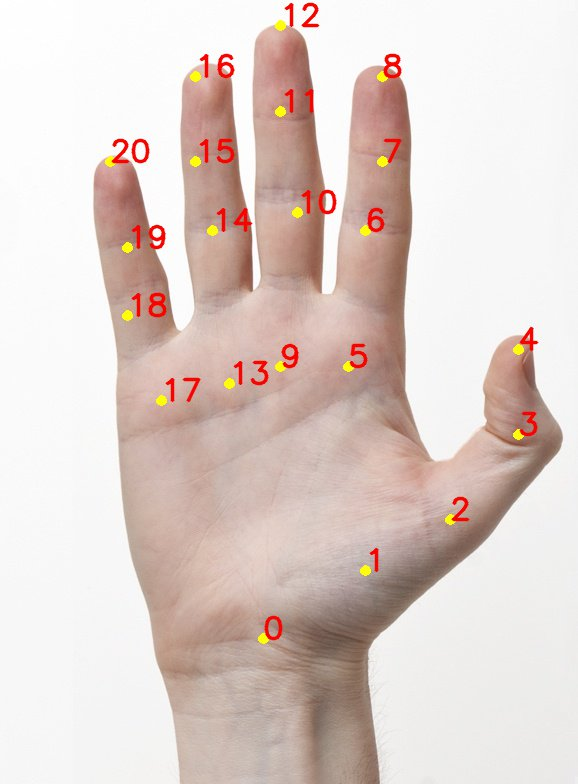
\includegraphics[width=0.4\textwidth,keepaspectratio]{figures/ru/handpose-demo-keypoints.jpg}
	\caption{Ключевые точки кисти руки}
	\label{fig:keypoints}
\end{figure*}

Далее для построения скелета необходимо соединить полученные точки в последовательностях, описанной в таблице \ref{tab:keypoints_skeleton}.

\begin{table}[h]
	\caption{\label{tab:keypoints_skeleton}Сравнение алгоритмов выделения источников}
	\begin{center}
		\begin{tabular}{|c|c|}
			\hline
			Ветвь скелета & Последовательность точек \\
			\hline
			Большой палец & 0 $\rightarrow$ 1 $\rightarrow$ 2 $\rightarrow$ 3 $\rightarrow$ 4 \\
			Указательный палец & 0 $\rightarrow$ 5 $\rightarrow$ 6 $\rightarrow$ 7 $\rightarrow$ 8 \\
			Средний палец & 0 $\rightarrow$ 9 $\rightarrow$ 10 $\rightarrow$ 11 $\rightarrow$ 12 \\
			Безымянный палец & 0 $\rightarrow$ 13 $\rightarrow$ 14 $\rightarrow$ 15 $\rightarrow$ 16 \\
			Мизинец & 0 $\rightarrow$ 17 $\rightarrow$ 18 $\rightarrow$ 19 $\rightarrow$ 20 \\
			\hline
		\end{tabular}
	\end{center}
\end{table} 

В ходе экспериментов было выявлена проблема с нахождением ключевых точек. На некоторых изображениях алгоритм либо не находил точки вообще, либо находил не полное их количество.